\chapter{Casos de uso}

Quando qualquer sistema é desenvolvido, este visa tornar possível diferentes
casos de uso, sendo estes realizados por um ou mais atores. Estes atores que
interagem diretamente com o sistema possuem requisitos que o sistema tem que
cumprir, isto é, funcionalidades que o sistema tem que possuir de modo a poder
responder às suas necessidades. Como tal, é necessário um levantamento destes
requisitos, de modo a melhor desenvolver o sistema para responder às
necessidades dos seus utilizadores.

Deste modo, neste capítulo iremos não só apresentar os atores que irão
interagir com o sistema, mas também os diversos usos que estes utilizadores
darão ao sistema, bem como os diversos requisitos que o mesmo tem de cumprir.

\section{Atores}

Como já foi referido, a criação de \emph{APIs GSMA Open Gateway} visa facilitar
a utilização programática dos diversos recursos e funcionalidades que a rede
\emph{5G} consegue oferecer. Deste modo, o sistema possui 2 atores distintos.
\begin{itemize} \item \textbf{Operador de rede} - O primeiro ator a interagir
	      com o sistema é o operador de rede, que fornece as APIs a diversos outros
	      negócios para que estes possam interagir com a rede programaticamente. No
	      entanto, tendo em consideração que as APIs desenhadas pelo \emph{GSMA Open
		      Gateway} são consideravelmente mais simples que as definidas pelo
	      \emph{3GPP}, um operador de rede pode também utilizar estas APIs para gerir a
	      própria rede.

	\item \textbf{\emph{Vertical
			      Clients}}\footnote{\url{https://5g-ppp.eu/verticals/}} - O segundo ator a
	      interagir com o sistema é na realidade o seu público alvo. Diversos
	      negócios que desenvolvem um conjunto de produtos que interagem com a rede.
	      Estes negócios utilizaram as APIs definidas pelo \emph{GSMA Open Gateway}
	      para não só oferecerem um maior leque de funcionalidades aos seus
	      utilizadores, como também para fazer um conjunto de verificações, de modo a
	      garantir a correta utilização e desempenho dos seus produtos. \end{itemize}

\section{Casos de Uso}

Os dois atores apresentados na secção anterior possuem diversos casos de uso.
Estes são apresentados no diagrama seguinte.

\begin{figure}[H] \centerline{
		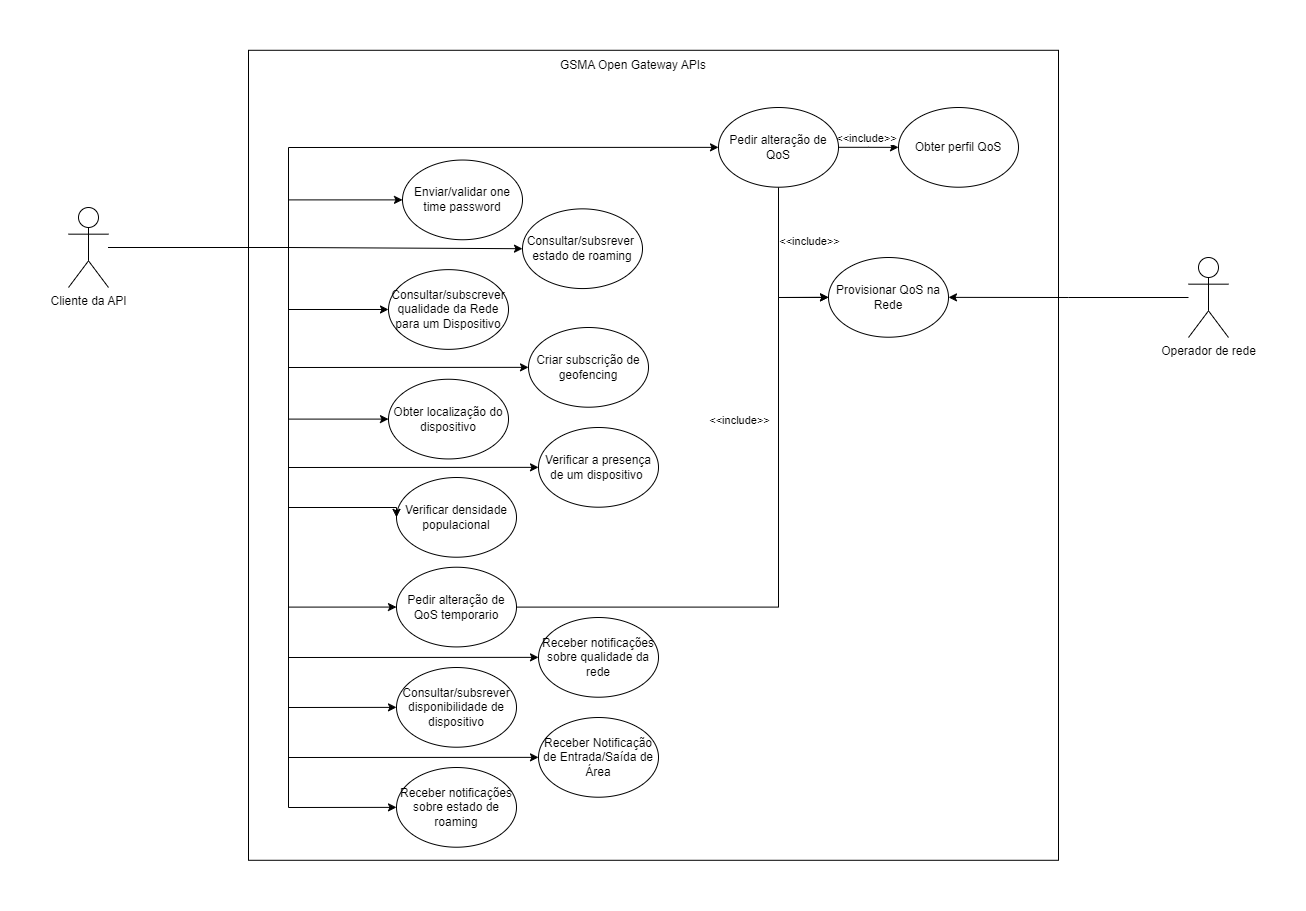
\includegraphics[width=20cm]{figs/use_case_diagram.png} } \caption{Diagrama de
		Casos de Uso} \end{figure}

\begin{itemize} \item \textbf{Operador de rede}

	      O operador de rede, apesar de poder interagir diretamente com o \emph{core
		      5G}, pode utilizar as APIs que disponibiliza para mais facilmente gerir a
	      qualidade de serviço da sua rede

	\item{\textbf{Cliente da API}}

	      Os clientes das APIs são os diversos negócios que pretendem
	      programáticamente modificar a rede, ou para oferecer melhores
	      produtos/serviços aos seus clientes, ou para manipular uma rede interna
	      para melhor se adaptar às suas necessidades. Utilizando as APIs definidas
	      pelo \emph{GSMA Open Gateway}, os diversos negócios podem:
	      \begin{enumerate} \item Enviar/Validar One Time Passwords (OTPs), para (por
		            exemplo) verificar a validade de um número de telefone via SMS \item
		            Consultar ou subscrever o estado do roaming, de modo a ser possível
		            verificar se um dispositivo se encontra em outro país. \item Consultar
		            e/ou subscrever a qualidade da rede para um determinado dispositivo, de
		            modo a saber se os requisitos de rede para a aplicação podem ser
		            alcançados, caso seja subscrito, sempre que exista uma alteração na
		            qualidade será enviada uma notificação.

		      \item Obter a localização de um dado dispositivo \item Verificar a
		            presença de um dispositivo, isto é, verificar se um determinado
		            dispositivo se encontra dentro da área definida. \item Verificar a
		            densidade populacional numa dada zona \item Pedir uma alteração de QoS,
		            temporário ou não, devido à necessidade de uma largura de banda maior.
		      \item Receber notificações sobre o estado da rede \item Receber
		            notificações relativas à entrada ou saída de um dispositivo de uma dada
		            área \item Subscrever/Consultar a disponibilidade de um dispositivo
	      \end{enumerate} \end{itemize}
